\documentclass[pdftex,a4paper,DIV15]{scrartcl}

\usepackage{cmap}
\usepackage[utf8]{inputenc}
\usepackage[utf8]{inputenc}
\usepackage[T1]{fontenc}
\usepackage[francais]{babel}
\usepackage{graphicx} 
\usepackage{adjustbox}
\usepackage{fancyref}
\usepackage{hyperref}
\usepackage{url}

\usepackage{url} 
\usepackage{array}
\usepackage{amsmath}
\usepackage{booktabs}
\usepackage{paralist}
\usepackage{hyperref}

\hyphenation{Map-Reduce}

\title{
CES Data Scientist - PageRank Exam}
\author{Youcef KACER (\texttt{youcef.kacer@telecom-paristech.fr})}


\begin{document}

\maketitle


\begin{description} % listes descriptives

\item[Exercise 1 :] We expose here after the system of linear equations that solves PageRank scores associated to graph $G$ ($r_{i}$ being PageRank score for page $i$):

\begin{eqnarray*} % systeme d'equation
r_1 &=& r_4\\
r_2 &=& 1/2*r_1\\
r_3 &=& 1/2*r_1 + r_2\\
r_4 &=& r_3\\
1   &=& r_1 + r_2 + r_3 + r_4
\end{eqnarray*}

We can solve manually the system :

\begin{eqnarray*} % systeme d'equation
r_1 &=& r_3\\
r_1 &=& r_4\\
r_2 &=& 1/2*r_1 \\
1   &=& 7/2*r_1
\end{eqnarray*}

\begin{eqnarray*} % systeme d'equation
r_1 &=& 2/7\\
r_2 &=& 1/7\\
r_3 &=& 2/7\\
r_4 &=& 2/7
\end{eqnarray*}
\\

Otherwise, we can solve the system using previous PageRank lab using MapReduce. We just need to adapt \begin{itshape}edge\_list.txt\end{itshape} to the graph $G$. 
In this file, each line represents a page indice and the page indices it links to :\\

1 2 3\\
2 3\\
3 4\\
4 1\\

We have run our python map/reduce implementation of PageRank. We use a teleport coefficient of $0.75$, and an error criteria of $0.01$. Figure \ref{mapreduce} shows correspoding standard output with 
PageRank scores results at the end.

\begin{figure}[H]
\begin{center}
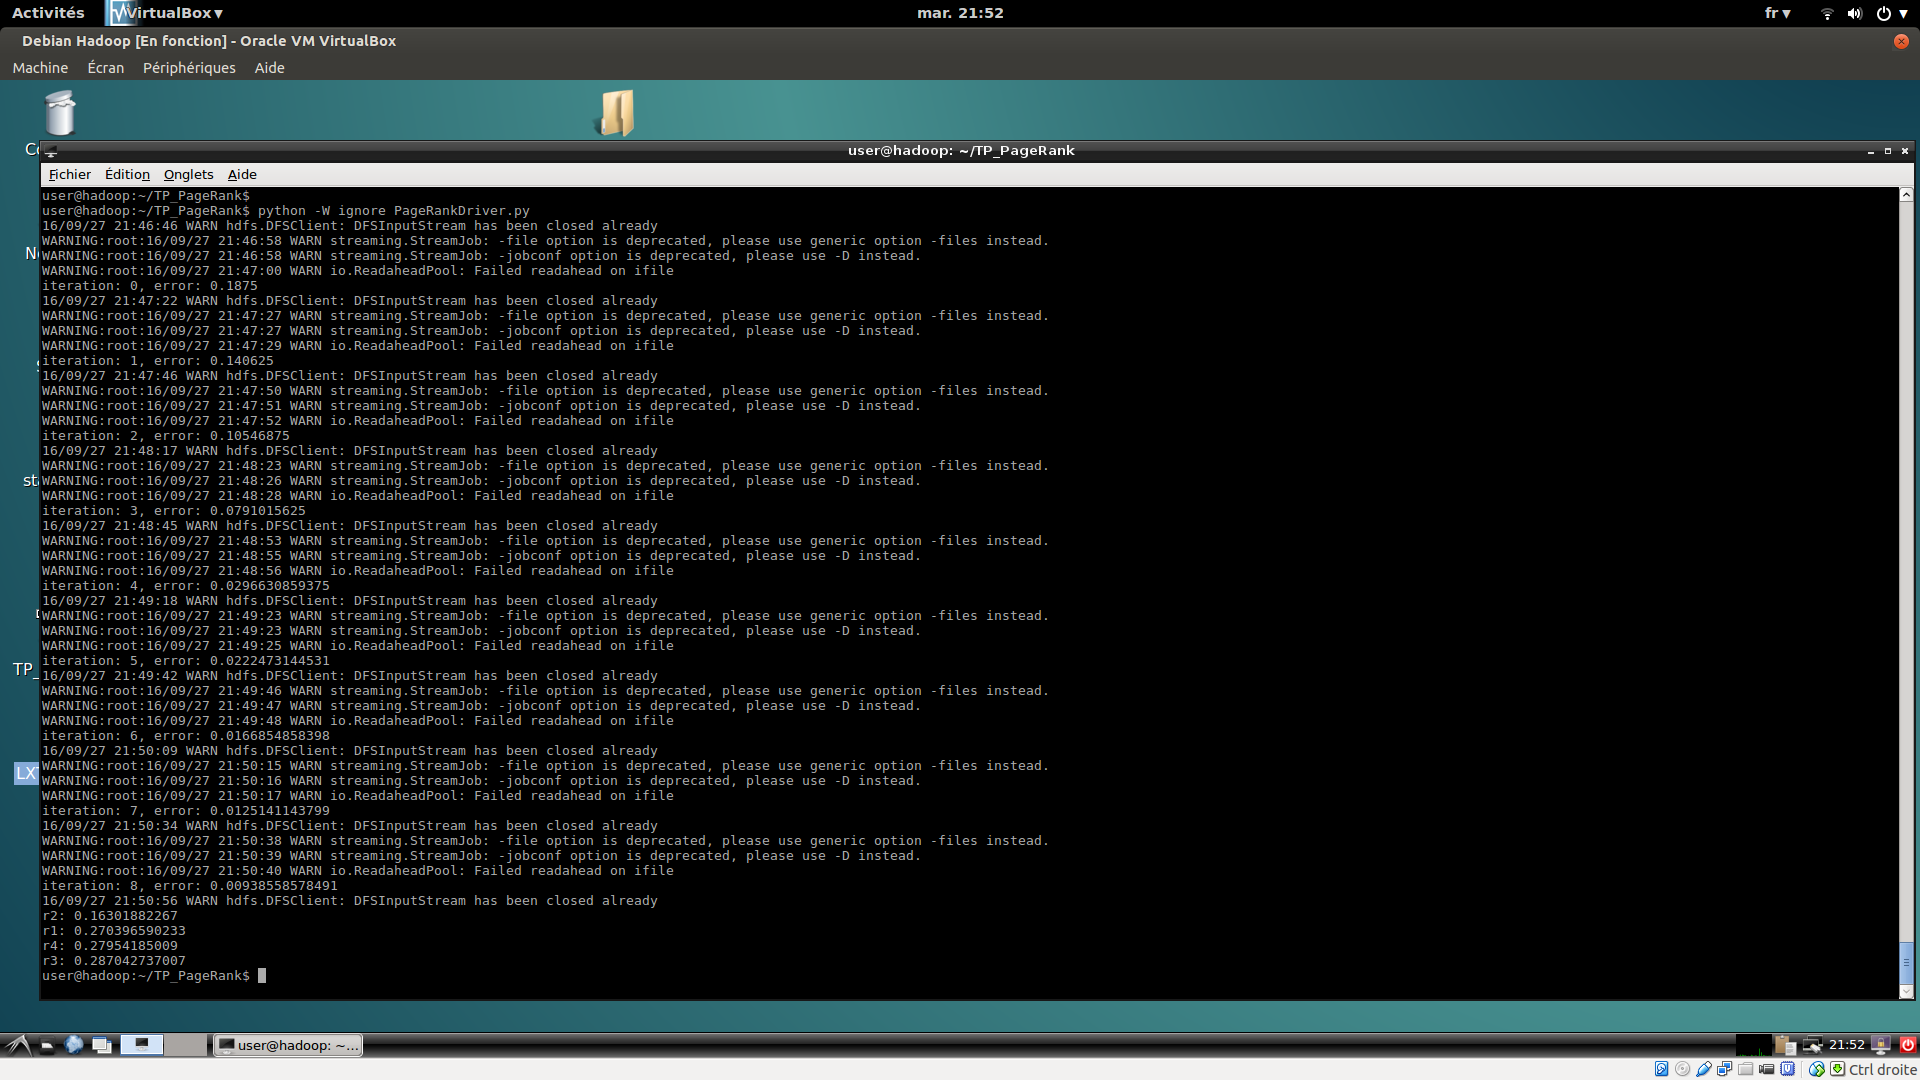
\includegraphics[scale=0.2]{images/mapreduce.png}
\end{center}
\caption{Python map/reduce for PageRank scores associated to graph $G$}
\label{mapreduce}
\end{figure}

\clearpage

\item[Exercise 2 :] Suppose we have a file containing integers with theirs indices as follow :\\

$i$ $n$\\
0 256 \\
1 35\\
2 4122\\
3 96\\
...\\

We present here after a pseudo-code for map/reduce function to find maximum value of this list of integers :\\

\begin{verbatim}
map(key=i,value=n)
{
  return 0,n
}

reduce(key,values) // values is an array containing all the integers because 
{                  // map has emitted each of them with the same key (0).
  MAX = MIN_POSSIBLE_VALUE
  for n in values
  {
    if n>max
    {
      max = n
    }
  }
  return max
}
\end{verbatim}

\item[Exercise 3 :] 

The keyword \begin{itshape}yield\end{itshape} is very useful to read data that are too big to fit in memory (RAM). Thus, we read those data directly from hard disk piece by piece.
For example, one can read a big .csv file line by line (or lines block by lines block). So, not all the data are in memory but only a piece at once. This is well suitable in
Map to provide large quantity of pairs (key,value), one by one into main memory of nodes.\\

\item[Exercise 4 :] 

\begin{itemize}

\item[1.] \textbf{True.}\\
\\
You can make parallel each element computation of vector result. We show here after a Map/Reduce implementation
for multiplying matrix $M_{i,j}$ ($i$ being line indice, $j$ row indice) by vector $V_{j}$
\begin{verbatim}
map(key=(i,Vj),value=Mij)
{
  yield i,Mij*Vj
}
reduce(key=k,value=v)
{
  sum = 0
  for p in v
  {
    sum = sum + p
  }
  yield k,sum
}
\end{verbatim}

\\
\item[2.] \textbf{False.}\\
\\
At each iteration, communication between nodes takes time, so too much iterations make the whole process slow.
\item[3.] \textbf{True.}\\
\\
The number of iterations needed for PageRank computation is 100, even smaller (10 as we experimented in our wikipedia lab).
\item[4.] \textbf{False.}\\
\\

\item[5.] \textbf{False.}\\
\\
Map/Reduce works efficiently in batch mode, not in streaming mode.
\end{itemize}

\end{description}

\end{document}